\documentclass[t, screen, aspectratio=43]{beamer}
\usepackage[T1]{fontenc}
\usepackage[utf8]{inputenc}
\usepackage{epsf}
\usepackage{graphicx}
\usepackage{geometry}
\usepackage{tabularx}
\usepackage[table]{colortbl}
\usepackage{xcolor}
\usepackage{soul}
\usepackage[normalem]{ulem}
% Use the NTNU-temaet for beamer 
% \usetheme[style=ntnu|simple|vertical|horizontal, 
%     language=bm|nn|en, 
%     smalltitle, 
%     city=all|trondheim|alesund|gjovik]{ntnu2017}
\usetheme[style=helvet,language=en]{ntnu2017}

\usepackage[english]{babel}
\usepackage[style=numeric,backend=biber,natbib=false,sorting=none]{biblatex}

\title[Short title]{Ultra-Low Power PLL for Wake-up Receiver Applications}
\subtitle{Specialization Project Progress - 7th Week}
\author[C Nielsen]{Cole Nielsen}
\institute[NTNU]{Department of Electronic Systems, NTNU}
\date{11 October 2019 (Calendar week 41)}
%\date{} % To have an empty date

\addbibresource{example.bib} % Add bibliography database

% Set the reference style to numeric.
% See here: http://tex.stackexchange.com/questions/68080/beamer-bibliography-icon
\setbeamertemplate{bibliography item}[text] 

% Set bibliography fonts to a small size.
\renewcommand*{\bibfont}{\footnotesize}

\begin{document}

\begin{frame}
	\titlepage%
\end{frame}

% Alternatively, special title page command to get a different background
% \ntnutitlepage

% #############################################################################
% Timeline
% #############################################################################
\begin{frame}
	\frametitle{Autumn Timeline}
	\begin{table}[htb!]
		\tiny
		\centering
		\vspace{-1em}
		\def\arraystretch{1.5}		
		\setlength\arrayrulewidth{0.75pt}
		\setlength{\tabcolsep}{1em} % for the horizontal padding
		\begin{tabular}{|l|l|l|l|}
			\hline 
			\rule[-1ex]{0pt}{2.5ex} \cellcolor{gray!40}\textbf{Week} & \cellcolor{gray!40}\textbf{Dates} &\cellcolor{gray!40}\textbf{Tasks} & \cellcolor{gray!40}\textbf{Outcomes}\\ 
			\hline 
			\rule[-1ex]{0pt}{2.5ex} \cellcolor{red!20}\textbf{36}& \cellcolor{red!20}2.9 - 8.9 & \cellcolor{red!20}Review PLL Design & \cellcolor{red!20}Refreshed Knowledge\\ 
			\hline 
			\rule[-1ex]{0pt}{2.5ex} \cellcolor{red!20}\textbf{37}& \cellcolor{red!20}9.9 - 15.9 & \cellcolor{red!20}Modeling/simulation (set up) & \cellcolor{red!20}--\\ 
			\hline 
			\rule[-1ex]{0pt}{2.5ex} \cellcolor{red!20}\textbf{38}& \cellcolor{red!20}16.9 - 22.9 & \cellcolor{red!20}Modeling/simulation &\cellcolor{red!20} TDC/DCO Requirements\\ 
			\hline 
			\rule[-1ex]{0pt}{2.5ex} \cellcolor{red!20}\textbf{39}& \cellcolor{red!20}23.9 - 29.9& \cellcolor{red!20}Modeling/simulation& \cellcolor{red!20}Loop Filter/Digital Algorithms\\ 
			\hline 
			\rule[-1ex]{0pt}{2.5ex} \cellcolor{red!20}\textbf{40}& \cellcolor{red!20}30.9 - 6.10& \cellcolor{red!20}Modeling/simulation& \cellcolor{red!20}{Loop filter, DCO, TDC, calibration}\color{black}\\ 
			\hline 
			\rule[-1ex]{0pt}{2.5ex} \cellcolor{green!20}\textbf{41}&\cellcolor{green!20}7.10 - 13.10&\cellcolor{green!20}Circuit Research &\cellcolor{green!20}DCO/Divider topologies, Ideal Virtuoso implementation\\ 
			\hline 
			\rule[-1ex]{0pt}{2.5ex} \textbf{42}& 14.10 - 20.10& Circuit Research & TDC/other topologies\\ 
			\hline 
			\rule[-1ex]{0pt}{2.5ex} \textbf{43}& 21.10 - 27.10& Circuit Implementation& Digital logic (schematic)\\ 
			\hline 
			\rule[-1ex]{0pt}{2.5ex} \textbf{44}& 28.10 - 3.11& Circuit Implementation& DCO (schematic)\\ 
			\hline 
			\rule[-1ex]{0pt}{2.5ex} \textbf{45}& 4.11 - 10.11& Circuit Implementation& Divider/other (schematic)\\ 
			\hline 
			\rule[-1ex]{0pt}{2.5ex} \textbf{46}& 11.11 - 17.11& Circuit Implementation (TDC)& \\ 
			\hline 
			\rule[-1ex]{0pt}{2.5ex} \textbf{47}& 18.11 - 24.11& Circuit Implementation (TDC)& TDC (schematic)\\ 
			\hline 
			\rule[-1ex]{0pt}{2.5ex} \textbf{48}& 25.11 - 1.12& Full Circuit testing & Testbenches, find bugs, design fixes\\ 
			\hline 
			\rule[-1ex]{0pt}{2.5ex} \textbf{49}& 2.12 - 8.12& Full Circuit testing& Design Fixes/iteration\\ 
			\hline 
			\rule[-1ex]{0pt}{2.5ex} \textbf{50}& 9.12 - 15.12& --& --\\ 
			\hline 
		\end{tabular}
		\begin{flushleft}\textbf{Legend:} \colorbox{red!20}{\textbf{Done}} \colorbox{green!20}{\textbf{Current}}  \colorbox{blue!20}{\textbf{Revised}}
		% *I will write the report simultaneously with the work.
		\end{flushleft}
		% \caption{Assigned specifications for branch line hybrid design.}
		% \label{asgn_specs}
	\end{table}   
\end{frame}


% #############################################################################
% This week
% #############################################################################

\begin{frame}
	\frametitle{Timeline Tasks}
	\begin{block}{This week}
		\begin{itemize}
			\footnotesize
			\item \textbf{Simulation of PLL}
			\begin{itemize}
				\footnotesize
				\item Finalized design of loop filter.
				\item Made script to compute filter coefficients for difference equation.
				\item Made new Python PLL simulation, completely in phase domain.
				\item Wrote Verilog module that implements loop filter.
				\item Working on schematic-based implementation of ideal PLL in Virtuoso...
			\end{itemize} 
			\item \textbf{DCO/Divider topologies}:
			\begin{itemize}
				\footnotesize
				\item Considered LC versus ring oscillator.
				\begin{itemize}
					\scriptsize
					\item Power limitations
					\item Start up time, tuning
				\end{itemize}
				\item Divider topologies
				\begin{itemize}
					\scriptsize
					\item Synchronous counter (replaces divider and TDC)
					\item $2^{N}$ to $2^{N-1}$ multimodulus with N chained 2/3 dual-modulus dividers.
					\item TSPC FF's to save power. 
				\end{itemize}
			\end{itemize} 
		\end{itemize}    
	\end{block}
\end{frame}

% #############################################################################
% sim/modeling approach
% #############################################################################

\begin{frame}
	\frametitle{PLL Simulation}
	\begin{block}{Final loop filter}
		\center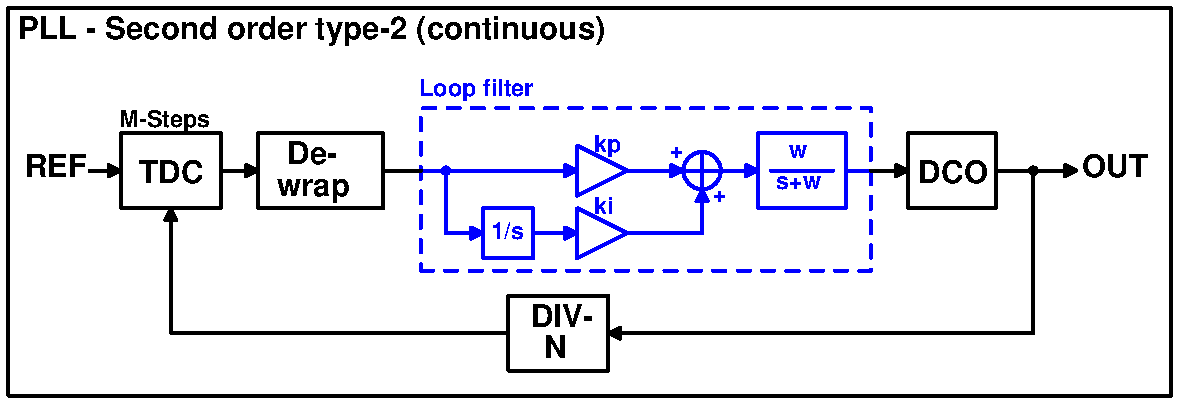
\includegraphics[width=0.6\textwidth, angle=0]{pll_sec_order_type2.pdf}
		\begin{itemize}
			\scriptsize
			\item Proportional-integral with added pole. Equal to second order type-2 (i.e. charge pump) PLL. (PI is chosen for no tracking error).
			\item Additional pole yields more favorable oscillator and TDC noise characteristics.
			\item \textbf{Not} second order, really three poles and one zero (open loop A(f) shown below).
			\begin{itemize}
				\scriptsize
				\item Computationally optimize loop filter transfer function so closed loop response approximates desired second order transfer function.
			\end{itemize}		
		\end{itemize} 
		\scriptsize	
		\begin{equation}
			A(s) = \frac{K}{s^2}\cdot\frac{(s/\omega_z + 1)}{(s/\omega_p + 1)}
		\end{equation}
	\end{block}
\end{frame}

\begin{frame}
	\frametitle{PLL Simulation}
	\begin{block}{Computation of discrete filter.}
		\center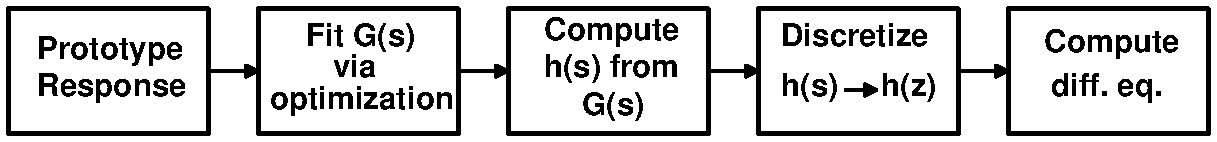
\includegraphics[width=0.8\textwidth, angle=0]{filter_coef_algorithm.pdf}
		\begin{itemize}
			\scriptsize
				\item \textbf{Goal:} Convert prototype second order response as defined by $\omega_n,\zeta$ and translate to a difference equation implementable in digital logic.
				\begin{itemize}
				\scriptsize
				\item PLL closed loop response G(s) is fit to the prototype response using gradient descent optimization of the parameters of A(s):
				\item PLL open loop response A(s) is computed from G(s). The loop filter response h(s) is comuted from A(s)
				\item h(f) is discretized as h(z), h(z) is translated into a difference equation y[n].
				\item Difference equation is implemented as multipliers, adders and registers.
			\end{itemize}
		\end{itemize} 	
		\scriptsize
		\begin{equation}
			G(s) = \frac{A(s)}{1+A(s)}, \hspace{1em} A(s) = \frac{M}{N}\frac{K_{DCO}}{s}h(s), \hspace{1em}h(s) = \frac{k_i}{s}\frac{s/\omega_z + 1}{s/\omega_p + 1}, \hspace{1em}\omega_z = \frac{k_i}{k_p}
		\end{equation}
	\end{block}
\end{frame}

\begin{frame}
	\frametitle{PLL Simulation}
	\begin{block}{Discrete time implementation.}
		\scriptsize
		\center\center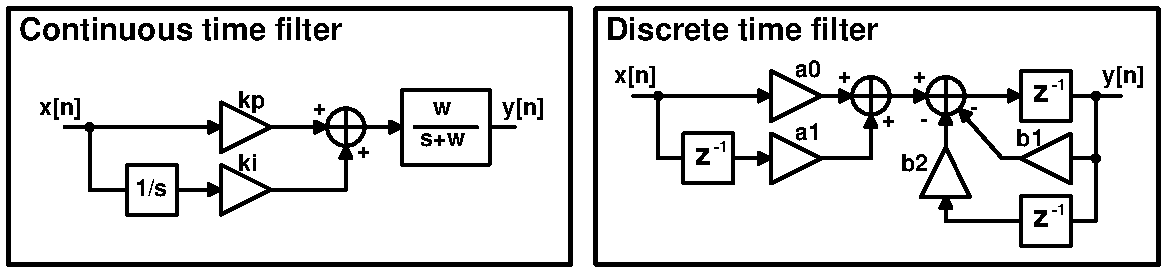
\includegraphics[width=1\textwidth, angle=0]{filter_arch.pdf}
		\vspace{-2em}
		\begin{multline}
			y[n] = x[n]\frac{K_i\omega_pT}{\omega_z}\frac{1+\omega_zT}{1+\omega_pT} - x[n-1]\frac{K_i\omega_pT}{\omega_z}\frac{1}{1+\omega_pT} + y[n-1]\frac{2+\omega_pT}{1+\omega_pT} - y[n-2]\frac{1}{1+\omega_pT}\\
			= a_0x[n] + a_1x[n-1] - b_1y[n-1] - b_2x[n-2] 
		\end{multline}
		\vspace{-2em}
		\begin{itemize}
			\scriptsize
			\item Implementation requires:
			\begin{itemize}
				\scriptsize
				\item \textbf{3 registers} (delay elements)
				\item \textbf{4 multipliers}
				\item \textbf{3 adders}
			\end{itemize}
		\end{itemize} 	
	\end{block}
\end{frame}

\begin{frame}
	\frametitle{PLL Simulation}
	\begin{block}{Example filter.}
		\scriptsize
		\begin{itemize}
			\scriptsize
			\item Using the described method, a filter was fitted to a 50 kHz bandwidth and $\zeta \approx 0.7$, for a 2.4 GHz PLL with 16 MHz reference and 64 TDC steps.
			\item Fitted response is close to protoype, but with a benefit:
			\begin{itemize}
				\scriptsize
				\item DCO noise is attenuated by 40 dB/decade below loop bandwidth (versus 20 for prototype filter)
			\end{itemize}
			\hspace{-5em}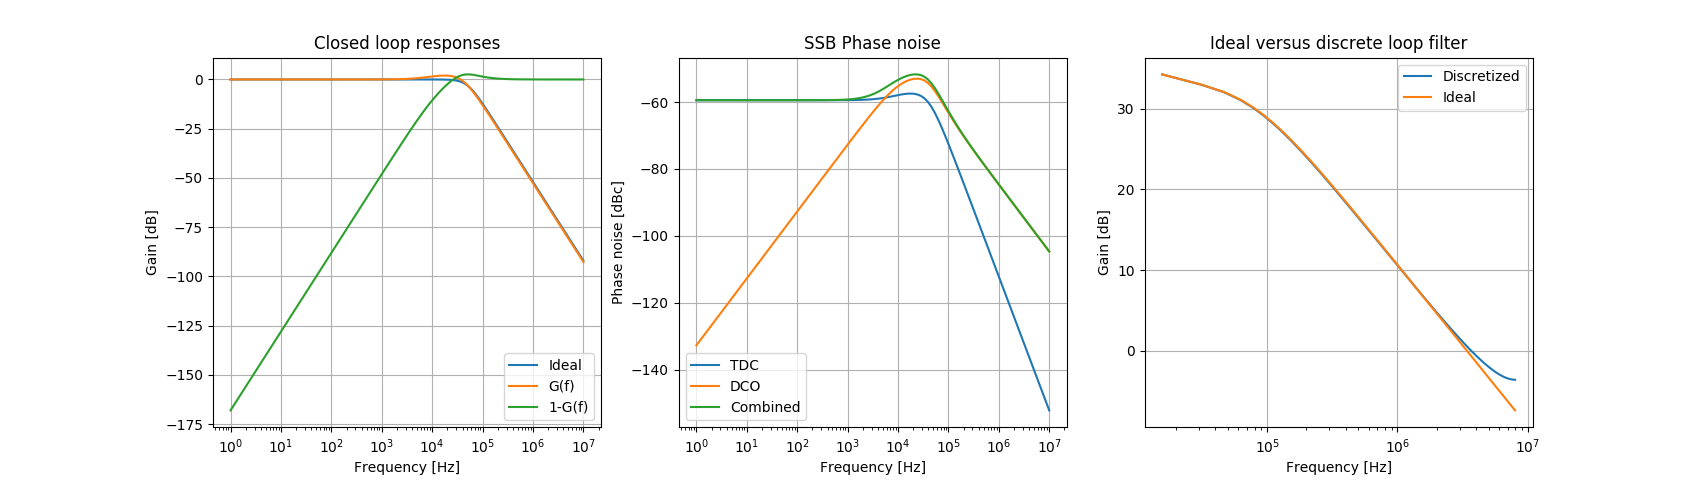
\includegraphics[width=1.1\textwidth, angle=0]{pll_xfer_sim.png}
		\end{itemize} 	
	\end{block}
\end{frame}

\begin{frame}
	\frametitle{PLL Simulation}
	\begin{block}{Python simulation results.}
	\begin{minipage}{3cm}
		\begin{itemize}
			\tiny
			\item Modified Python simulation to be 100\% phase domain, for better phase noise resolution.
			\item Loop filter design successful - architecture achieves lock and rejects phase noise.
			\item There is a error in my filter design math/code, PLL bandwidth in simulation is 5x smaller than intended.
		\end{itemize} 	
	\end{minipage}
	\begin{minipage}{8cm}
		\center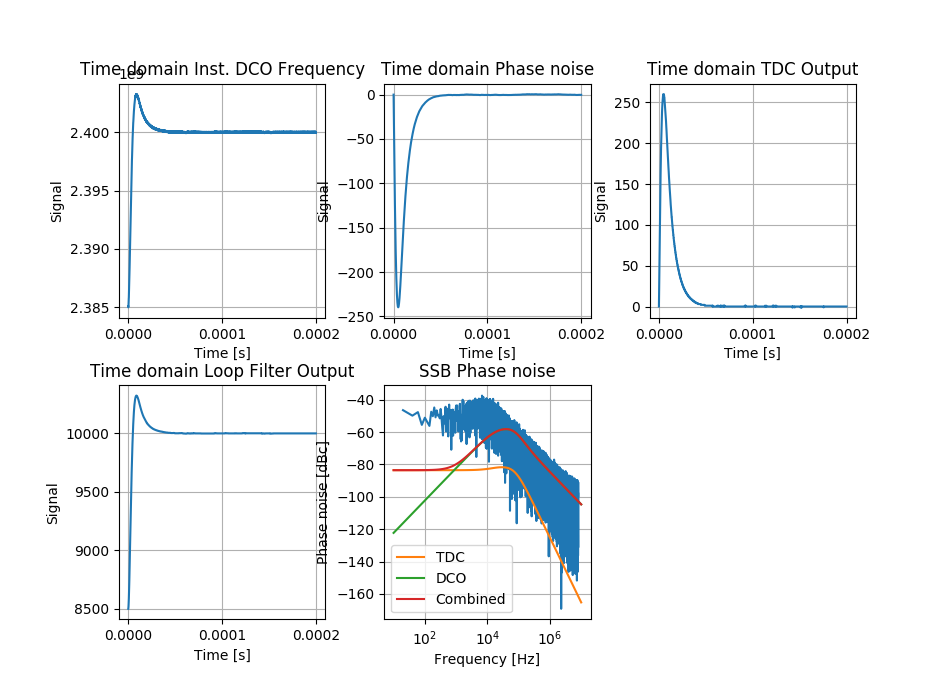
\includegraphics[width=1.1\textwidth, angle=0]{simulation_phase_domain.png}
	\end{minipage}
	\end{block}
\end{frame}

\begin{frame}
	\frametitle{PLL Simulation}
	\begin{block}{Loop filter Logic Implementation.}
		\center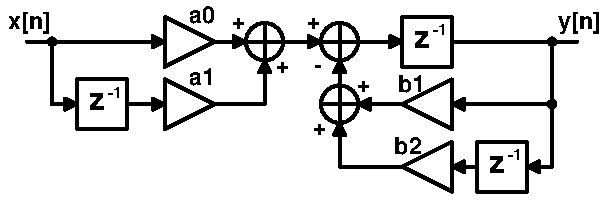
\includegraphics[width=0.4\textwidth, angle=0]{discrete_filter2.pdf}
		\begin{itemize}
			\scriptsize
			\item Translation to hardware:
			\begin{itemize}
				\scriptsize
				\item Delay blocks are implemented as registers (3 total)
				\item Gain blocks are implemented as multipliers (4 total)
				\item Sums are adders (3 total)
			\end{itemize}
			\item Decide bits of resolution for datapath on TDC/DCO resolution and gain coefficients.
			\item Will re-evaluate resolution based on power consumption after synthesis/place+route. 
		\end{itemize} 	
	\end{block}
\end{frame}

\begin{frame}
	\frametitle{PLL Simulation}
	\begin{block}{Resolution of datapath.}
		\begin{itemize}
			\scriptsize
			\item Will use signed integers representing fixed point values.
			\item TDC resolution ($N_{TDC}$) defines required number of integer bits on input.
			\item DCO resolution ($N_{DCO}$) defines required number of integer bits on output.
			\item Fractional bits needed is (for gains, but applied to all):
			\begin{equation}
				\textnormal{Fractional bits} > \lceil -\log_2(a_0+a_1) \rceil
			\end{equation}
			\item Integer bits needed for gain coefficients:
			\begin{equation}
				\textnormal{Integer bits} > \lceil1 -\log_2(\max(|\{a_0, a_1, b_1, b_0\}|)) \rceil
			\end{equation}
			\item It is expected that the minimum \textit{required} resolutions will then be:
			\begin{itemize}
				\scriptsize
				\item Input  : 6 integer bits, 0 fractional
				\item Gains  : 2 integer bits, 9 fractional
				\item Output : 10 integer bits, 0 fractional
			\end{itemize}
			\item (The filter coefficients $a_0, a_1, b_1, b_0$ are on the order of 1)
		\end{itemize} 	
	\end{block}
\end{frame}




\begin{frame}
	\frametitle{PLL Simulation}
	\begin{block}{Verilog implementation.}
	\begin{minipage}{5cm}
		\begin{itemize}
			\scriptsize
			\item Currently more bits than needed. Will make more efficient implementation later.
			\item Use fixed point with 4 integer bits + 12 fractional bits for filter coefficients.
			\item Input and output are 16 bit signed integers.
			\item Will multiplication/addition here be handled in synthesis, or do I need to do this?
		\end{itemize} 	
	\end{minipage}
	\begin{minipage}{6cm}
		\vspace{1em}
		\hspace{1em}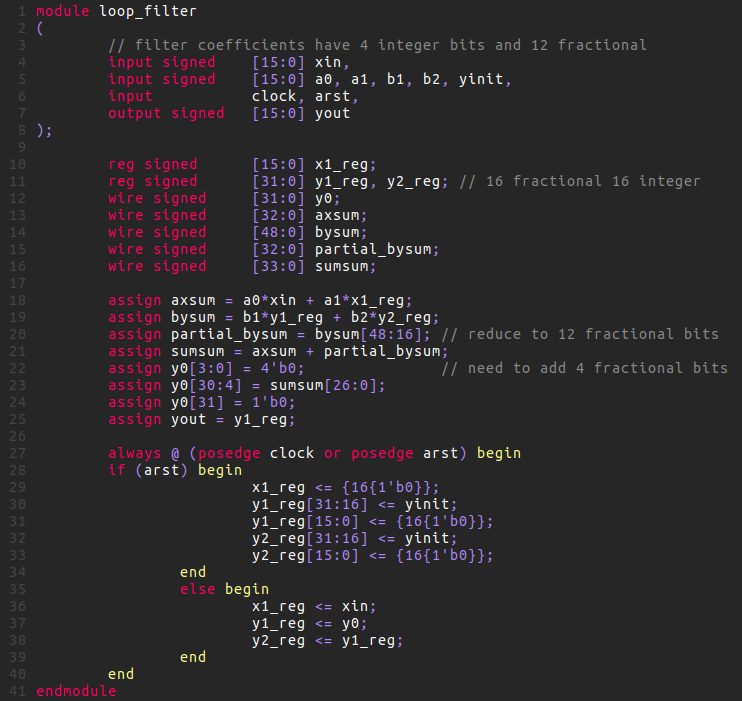
\includegraphics[width=1\textwidth, angle=0]{verilog_module.png}
	\end{minipage}
	\end{block}
\end{frame}




\begin{frame}
	\frametitle{PLL Simulation}
	\begin{block}{Ideal PLL - Virtuoso schematic.}
		\begin{itemize}
			\scriptsize
			\item Have loop filter (imported from Verilog module) and DCO implemented.
			\item Need to implement divider/TDC in Verilog (couldn't be easily done with ahdlLib).
			\begin{itemize}
				\scriptsize
				\item Wasted quite a bit of time re-learning Verilog, so ran out of time for this.
			\end{itemize}
			\vspace{-0.5em}
			\center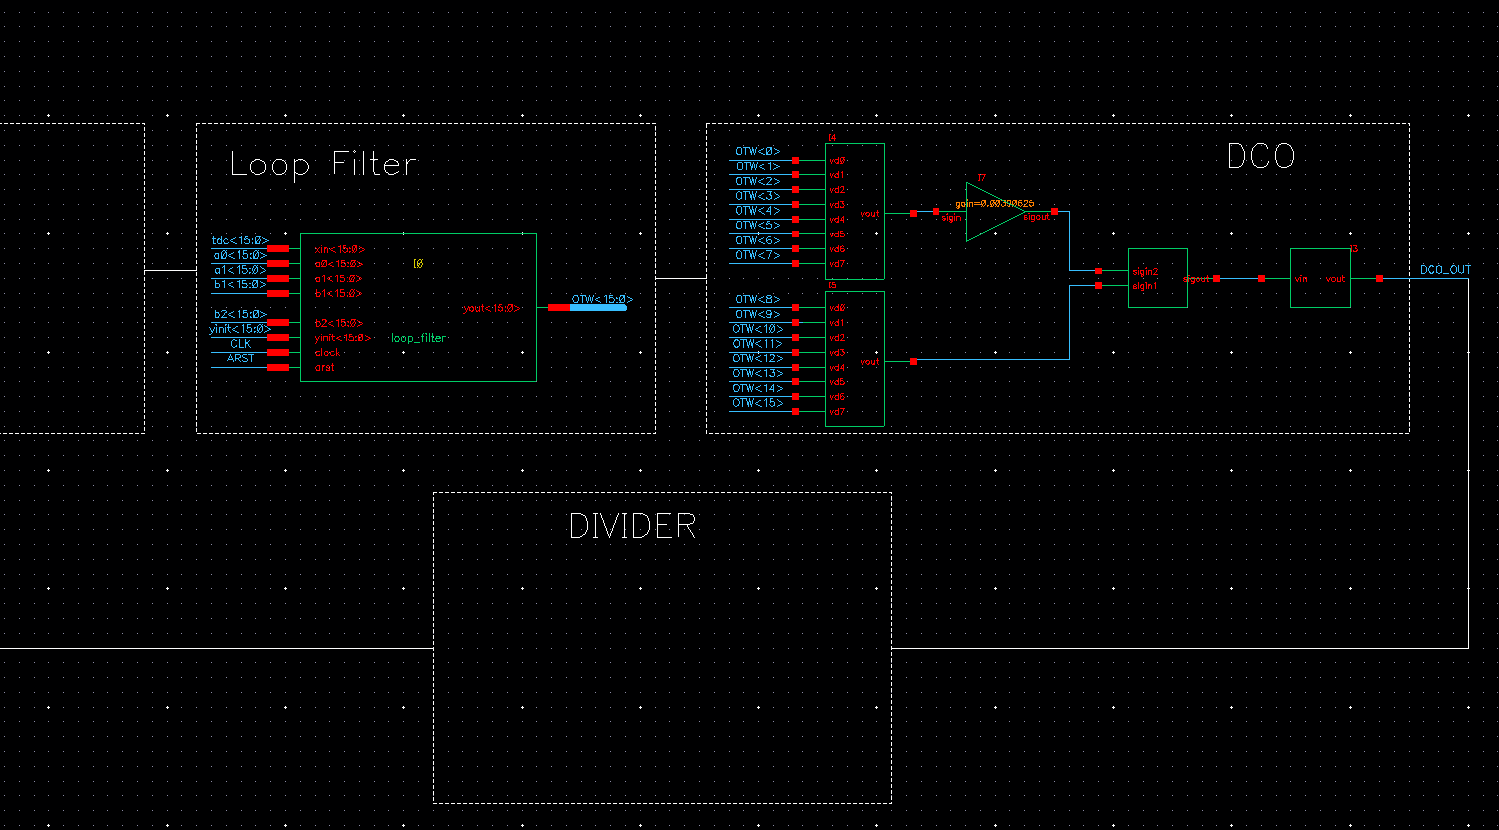
\includegraphics[width=0.8\textwidth, angle=0]{pll_virtuoso.png}
			\vspace{-0.5em}
		\end{itemize} 	
	\end{block}
\end{frame}


\begin{frame}
	\frametitle{DCO topologies}
	\begin{block}{LC Oscillator versus Ring Oscillator.}
	\begin{minipage}{6cm}
		\vspace{1em}
		\begin{itemize}
			\scriptsize
			\item \textbf{LC Oscillator}.
			\begin{itemize}
				\scriptsize
				\item Inductor Q and $g_m/I_D$ doesn't scale well with process.
				\item Thus minimum $I_D$ for $A_V = g_mR_p > 1$ needed for startup doesn't scale well.
				\item At 2 GHz, need >$60 \mu W$ minimum to satisfy start-up conditions. Power increased by extra phases and margin needed to account for variation.
				\item Start-up time $>>1\mu s$.
				\item Requires level control, buffering to drive mixers.
				\item \textbf{Good phase noise.}
			\end{itemize}
		\end{itemize} 	
		\end{minipage}
		\begin{minipage}{5cm}
				\vspace{1em}
			\tiny
			\textbf{2 GHz oscillator minimum power versus process node scaling analysis from pg. 89 of  [1].}
			\center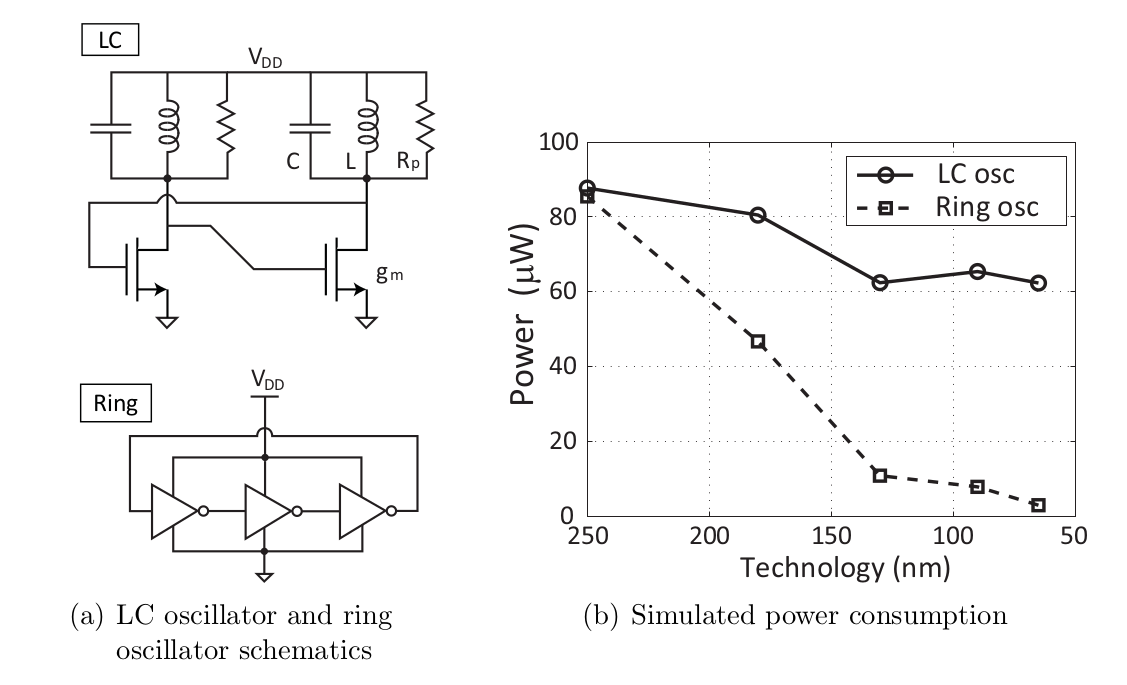
\includegraphics[width=1\textwidth, angle=0]{lc_vs_ro_power.png}
		\end{minipage}
	\end{block}
\end{frame}

\begin{frame}
	\frametitle{DCO topologies}
	\begin{block}{LC Oscillator versus Ring Oscillator.}
	\begin{minipage}{6cm}
		\vspace{1em}
		\begin{itemize}
			\scriptsize
			\item \textbf{Ring oscillator}
			\begin{itemize}
				\scriptsize
				\item Ring oscillator power scales well with process node. In 20 nm can achieve 2 GHz oscillator with ca. $1 \mu W$
				\item Extra phases with little to no power penalty.
				\item Instant start-up.
				\item Can reset to known phase, which can be exploited in PLL for faster lock.
				\item Small area.
				\item \textbf{Bad phase noise (+20 dB vs LC).}
			\end{itemize}
		\item \textbf{Conclusion}: LC power prohibitive, have to use ring oscillator.
		\end{itemize} 	
		\end{minipage}
		\begin{minipage}{5cm}
				\vspace{1em}
			\tiny
			\textbf{Oscillator figure of merit comparison.}
			\center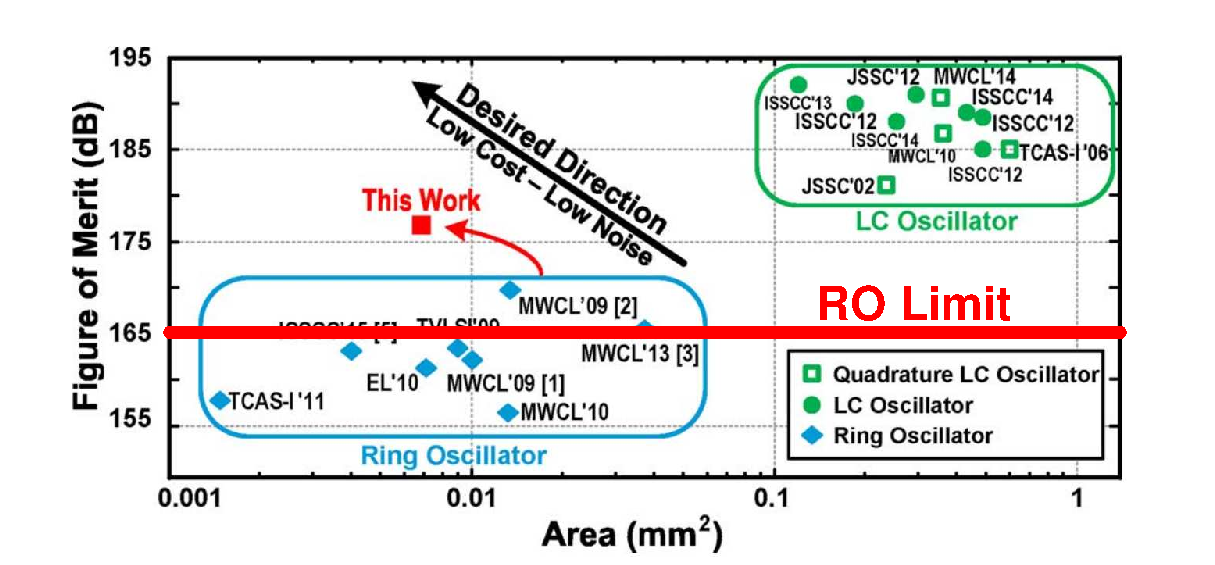
\includegraphics[width=1\textwidth, angle=0]{ro_perf.pdf}
		\end{minipage}
	\end{block}
\end{frame}

\begin{frame}
	\frametitle{DCO topologies}
	\begin{block}{Ring oscillator architecture.}
	\begin{minipage}{6cm}
		\vspace{1em}
		\begin{itemize}
			\scriptsize
			\item Proposed ring oscillator: pseudo-differential with back-gate control of frequency.
			\item Frequency tuning is highly linear with $V_{ctrl}$, allows for 0-$V_{DD}$ control range.
			\item Use DAC to set control voltage (10 bit?) for medium frequency tuning.
			\item Design for 10\% fractional tuning range, so 10 bits is 240 kHz/LSB at 2.4 GHz.
			\item Utilize 5-bit unit-capacitor based digital capacitor for fine tuning, approximately 7.5 kHz/LSB
			\item Need frequency step to be $<<$ PLL bandwidth (50 kHz).
		\end{itemize} 	
		\end{minipage}
		\begin{minipage}{5cm}
				\vspace{1em}
			\tiny
			\textbf{Pseudo-differential ring oscillator utilizing backgate-based coupling and frequency control.}
			\center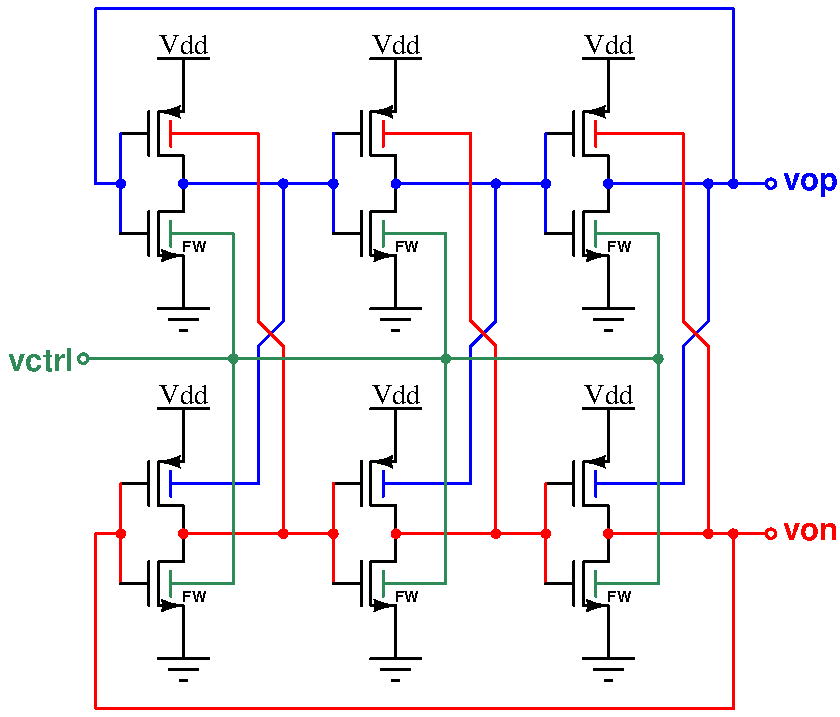
\includegraphics[width=1.0\textwidth, angle=0]{pseudodiff_ro.pdf}
		\end{minipage}
	\end{block}
\end{frame}

\begin{frame}
	\frametitle{DCO frequency tuning and $K_{DCO}$}
	\begin{block}{Backgate coupled pseudo-differential ring oscillator}
		\begin{itemize}
			\scriptsize
			\item The center frequency of the oscillator, with $V_{ctrl}=V_{DD}/2$:
			\tiny
		\begin{equation}
			f_{c} = \frac{\mu_nC_{ox}}{4\ln2NC}\left(\frac{W}{L}\right)_n\left[V_{DD}\left(\frac{7}{8\ln2}-1+\frac{\gamma}{2\ln2}-\frac{\gamma}{2}\right)-V_{t0}\left(\frac{1}{\ln2}-1\right)\right]
		\end{equation}
			\scriptsize
			\item The fractional tuning range of the oscillator is:
			\tiny
	\begin{equation}
		\frac{\Delta f}{f_c} = \frac{1}{2}\cdot\frac{\gamma V_{DD}\left( 1-\ln2 \right)}{V_{DD}\left(\frac{7}{8}-\ln2+\frac{\gamma}{2}-\frac{\gamma}{2}\ln2\right)-V_{t0}\left(1-\ln2\right)}
	\end{equation}	
			\scriptsize
			\item If a N-bit DAC is used to control the oscillator, the resulting DCO gain is therefore:
			\tiny
	\begin{equation}
		K_{DCO} = \frac{\Delta f}{2^{N_{DAC}}} = \frac{f_c}{2^{N_{DAC}+1}}\cdot\frac{\gamma V_{DD}\left( 1-\ln2 \right)}{V_{DD}\left(\frac{7}{8}-\ln2+\frac{\gamma}{2}-\frac{\gamma}{2}\ln2\right)-V_{t0}\left(1-\ln2\right)}
	\end{equation}	

		\end{itemize} 	
	\end{block}
\end{frame}


\begin{frame}
	\frametitle{Divider topologies}
	\begin{block}{Divider options.}
		\begin{itemize}
			\scriptsize
			\item Divider design is more trivial than the other components.
			\item \textbf{Synchronous counter.} 
			\begin{itemize}
				\scriptsize
				\item Use ripple counter + TSPC FF's for low power.
				\item Lower jitter due to being synchronous.
			\end{itemize}
			\item \textbf{Multi-modulus divider (asynchronous).}
			\begin{itemize}
				\scriptsize
				\item N chained 2/3 dual modulus dividers. 7 stage? 
				\item Tunable from $2^N$ to $2^{N+1}-1$. N = 7 yields 128-255 range for divider modulus.
			\end{itemize}
			\item Jitter compounds with divider chains, effect on phase noise???

			\vspace{-0.5em}
			\center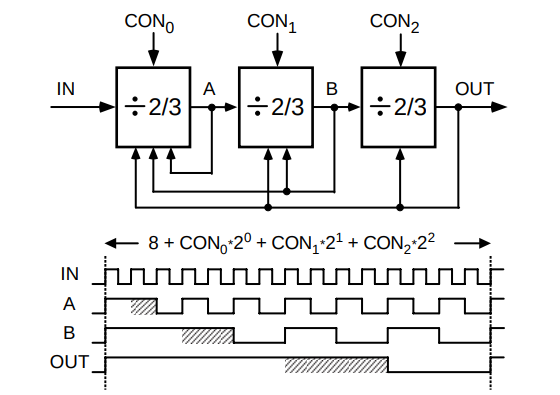
\includegraphics[width=0.3\textwidth, angle=0]{multimod_div.png}
			\vspace{-0.5em}
		\end{itemize} 	
	\end{block}
\end{frame}



% #############################################################################
% Loop Dynamics (continuous)
% #############################################################################

% \begin{frame}
% 	\frametitle{Loop Dynamics}
% 	\begin{block}{Still To Do}
% 		\vspace{-.2em}
% 		\begin{itemize}
% 			\footnotesize
% 			\item Standard approach to used mixed continuous/discrete time mathematical model for DPLL. 
% 			\item Plot of RO phase noise (typical)
% 			\item Automatic analysis of performance (lock detection, residual phase modulation, lock-in/pull-in range).
% 			\item Automatic optimization (using gradient descent) of PLL parameters?
% 			\item Z-domain modeling of loop? Develop (by hand) some ideal transfer funtions for loop.

% 		\end{itemize}    
% 	\end{block}
% \end{frame}

% #############################################################################
% Specification
% #############################################################################

\begin{frame}
	\frametitle{Specification (unchanged)\color{black}}
	\begin{block}{System Performance Targets}
		\scriptsize
		\begin{table}[h!]
			\centering
			\def\arraystretch{1.5}		
			\setlength\arrayrulewidth{0.75pt}
			\setlength{\tabcolsep}{1em} % for the horizontal padding
			\begin{tabular}{|l|r|l|l|}
				\hline 
				\rule[-1ex]{0pt}{2.5ex} \cellcolor{gray!40}\textbf{Parameter} & \cellcolor{gray!40}\textbf{Value} & \cellcolor{gray!40}\textbf{Unit }& \cellcolor{gray!40}\textbf{Notes}\\ 
				\hline 
				\rule[-1ex]{0pt}{2.5ex} \textbf{Frequency}  & 2.4-2.4835 & GHz & 2.4G ISM Band\\ 
				\hline 
				\rule[-1ex]{0pt}{2.5ex} \textbf{Ref. frequency} & 16 & MHz & Yields 6 channels \\ 
				\hline 
				\rule[-1ex]{0pt}{2.5ex} \textbf{Power} & $\leq$ 100  &$\mu$W & \\ 
				\hline 
				\rule[-1ex]{0pt}{2.5ex} \textbf{FSK BER} & $\leq$ 1e-2  & & 2FSK with $f_{dev}$=$\pm$250 KHz\\ 
				\hline 
				\rule[-1ex]{0pt}{2.5ex} \textbf{Initial Lock Time} & $\leq$ 50 & $\mu$s & Upon cold start \\ 
				\hline 
				\rule[-1ex]{0pt}{2.5ex} \textbf{Re-lock Time} & $\leq$ 5 & $\mu$s & Coming out of standby \\ 
				\hline 
				\rule[-1ex]{0pt}{2.5ex} \textbf{Bandwidth} & 50 & kHz & (nominally), tunable \\ 
				\hline 
			\end{tabular} 
			% \caption{Assigned specifications for branch line hybrid design.}
			% \label{asgn_specs}
		\end{table}   
		Additionally: PLL output should support IQ sampling at LO frequency.
	\end{block}    
\end{frame}

\begin{frame}
	\frametitle{Specification (unchanged)}
	\begin{block}{PLL Component Performance Targets}
		\scriptsize
		\begin{table}[h!]
			\centering
			\def\arraystretch{1.5}		
			\setlength\arrayrulewidth{0.75pt}
			\setlength{\tabcolsep}{1em} % for the horizontal padding
			\begin{tabular}{|l|r|l|l|}
				\hline 
				\rule[-1ex]{0pt}{2.5ex} \cellcolor{gray!40}\textbf{Parameter} & \cellcolor{gray!40}\textbf{Value} & \cellcolor{gray!40}\textbf{Unit }& \cellcolor{gray!40}\textbf{Notes}\\ 
				\hline 
				\rule[-1ex]{0pt}{2.5ex} \textbf{DCO LSB Resolution}  & $\leq$ 50  & kHz & Determined from quantization noise.\\ 
				\hline 
				\rule[-1ex]{0pt}{2.5ex} \textbf{DCO DNL} & < 1 & LSB & Ensures monotonicity \\ 
				\hline 
				\rule[-1ex]{0pt}{2.5ex} \textbf{TDC Resolution} & 0.95  & ns & \\ 
				\hline 
				\rule[-1ex]{0pt}{2.5ex} \textbf{TDC Resolution (bits)} &  6 &bits & \\ 
				\hline 
			\end{tabular} 
			% \caption{Assigned specifications for branch line hybrid design.}
			% \label{asgn_specs}
		\end{table}   
	\end{block}    
\end{frame}

% #############################################################################
% Architecture - block diagram
% #############################################################################

\begin{frame}
	\frametitle{Architecture (unchanged)}
	\begin{block}{Block Diagram}
	\center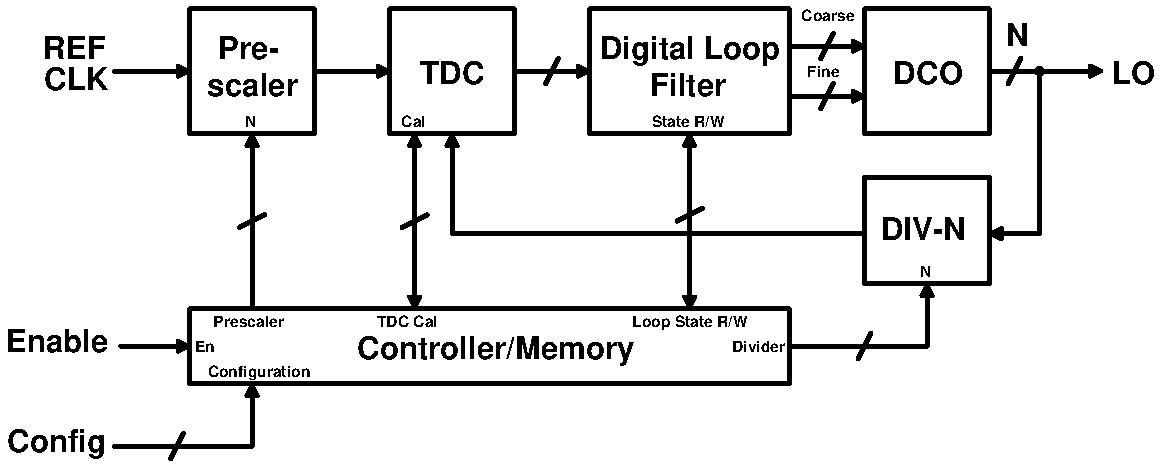
\includegraphics[width=0.75\textwidth, angle=0]{pll2.pdf}

	\end{block}
		\begin{block}{Power Targets}
		\vspace{-.1em}
		\begin{table}[htb!]
			\tiny
			\centering
			\def\arraystretch{1.5}		
			\setlength\arrayrulewidth{0.75pt}
			\setlength{\tabcolsep}{1em} % for the horizontal padding
			\begin{tabular}{|l|l|l|l|l|}
				\hline 
				\rule[-1ex]{0pt}{2.5ex} \cellcolor{gray!40}\textbf{DCO} & \cellcolor{gray!40}\textbf{TDC} & \cellcolor{gray!40}\textbf{Divider }& \cellcolor{gray!40}\textbf{Other} & \cellcolor{gray!40}\textbf{SUM} \\ 
				\hline 
				\rule[-1ex]{0pt}{2.5ex} 70 $\mu$W& 20 $\mu$W & 10 $\mu$W & $<<$ 1 $\mu$W & 100 $\mu$W\\ 
				\hline 
			\end{tabular} 
			% \caption{Assigned specifications for branch line hybrid design.}
			% \label{asgn_specs}
		\end{table}   
	\end{block}

\end{frame}


% #############################################################################
% project phases
% #############################################################################


\begin{frame}
	\frametitle{Project Phases}
	\begin{block}{Autumn 2019}
		\footnotesize
		\begin{itemize}
			\item System modeling and simulation.
			\begin{itemize}
				\footnotesize
				\item Learn PLL theory in detail
				\item Evaluate feasability of PLL architectures (counter, TDC-based)
				\item Determine requirements for TDC/DCO/Divider/logic (bits of resolution, accuracy etc) to meet PLL performance specifications.
				\item Determine digital logic for loop filter, validate stability and lock time performance.
			\end{itemize}
			\item Research ultra-low power circuit topologies to implement system components that will meet determined requirements.
			\item Translate component-level specifications into schematic-level circuit designs.
			\begin{itemize}
				\footnotesize
				\item Try, fail, try again until functional at schematic level.
				\begin{itemize}
					\footnotesize
					\item I expect the TDC to be difficult.
				\end{itemize}
			\end{itemize}      
		\end{itemize}
	\end{block}
\end{frame}

% #############################################################################
% Project phases slide 2
% #############################################################################


\begin{frame}
	\frametitle{Project Phases (continued)}
	\begin{block}{Spring 2020}
		\begin{itemize}
			\footnotesize
			\item Finalize schematic-level design.
			\item Estabilish thorough tests for PLL performance (automated?) to help in layout.
			\item Layout of PLL.
			\begin{itemize}
				\footnotesize
				\item Design iteration until design specs met.
				\item Probably very time consuming.
			\end{itemize}
			\item Full characterization/validation of design performance. 
			\begin{itemize}
				\footnotesize
				\item Comprehensive Corners/Monte-Carlo testing (time consuming??)
				\item More design iteration if new issues crop up...
			\end{itemize}
			\item Thesis paper writing.
		\end{itemize}
	\end{block}
\end{frame}

% #############################################################################
% References
% #############################################################################


\begin{frame}
	\frametitle{References}
		\scriptsize
		[1] "Ultra-Low Power Wake-Up Receivers for Wireless Sensor Networks", N. Pletcher, J.M Rabaey, 2008.\\
		\hspace{16pt}\url{http://www.eecs.berkeley.edu/Pubs/TechRpts/2008/EECS-2008-59.html}\\
		\vspace{1em}
		% [2] "Minimum Achievable Phase Noise of RC Oscillators",
	% Navid et al. 2005
\end{frame}


\end{document}
